\documentclass[12pt]{article}
\usepackage[margin=1in]{geometry} 
\usepackage{amsmath,amsthm,amssymb,amsfonts}
\usepackage{tabto}
\usepackage{hyperref}
\usepackage[linesnumbered,ruled]{algorithm2e}
\usepackage{wrapfig}
\usepackage[super]{nth}
\usepackage{needspace}
\usepackage[font=small]{caption, subcaption}
\usepackage[backend=biber]{biblatex}

% Spacers:
% BEGIN BLOCK------------------------------------------
% END BLOCK============================================


\usepackage{wrapfig}

\newcommand{\N}{\mathbb{N}}
\newcommand{\Z}{\mathbb{Z}}

% CUSTOM SETTINGS
% BEGIN BLOCK------------------------------------------
% For equation system alignment
\usepackage{systeme,mathtools}
% Usage:
%	\[
%	\sysdelim.\}\systeme{
%	3z +y = 10,
%	x + y +  z = 6,
%	3y - z = 13}


% For definitions
\newtheorem{defn}{Definition}[section]
\newtheorem{thrm}{Theorem}[section]

% For circled text
\usepackage{tikz}
\newcommand*\circled[1]{\tikz[baseline=(char.base)]{
            \node[shape=circle,draw,inner sep=0.8pt] (char) {#1};}}

\newenvironment{problem}[2][Problem]{\begin{trivlist}
\item[\hskip \labelsep {\bfseries #1}\hskip \labelsep {\bfseries #2.}]}{\end{trivlist}}
%If you want to title your bold things something different just make another thing exactly like this but replace "problem" with the name of the thing you want, like theorem or lemma or whatever
 
%used for matrix vertical line
\makeatletter
\renewcommand*\env@matrix[1][*\c@MaxMatrixCols c]{%
  \hskip -\arraycolsep
  \let\@ifnextchar\new@ifnextchar
  \array{#1}}
\makeatother 

% END BLOCK============================================

\newtheorem*{lemma}{Lemma} %added
\newtheorem*{result}{Result} %added
\newtheorem*{theorem}{Theorem} %added
\theoremstyle{definition}
\newtheorem*{solution}{Solution} %added
\theoremstyle{plain}

% HEADER
% BEGIN BLOCK------------------------------------------
\usepackage{fancyhdr}
 
%\pagestyle{fancy}
\fancyhf{}
\rhead{Bryan Greener}
\cfoot{\thepage}
% END BLOCK============================================
\bibliography{citations}
\begin{document}

\thispagestyle{empty}
\begin{center}
\begin{minipage}{0.75\linewidth}
	\centering
	
\includegraphics[width=0.35\linewidth]{wmulogo.png}\\
	%\rule{0.4\linewidth}{0.15\linewidth}\par
	\vspace{2cm}
	{\uppercase{\Large Feed Forward Neural Networks using Backpropagation and Gradient Descent\par}}
	\vspace{3cm}
	{\Large Bryan Greener\par}
	\vspace{3cm}
	{\Large Design and Analysis of Algorithms\par}
	\vspace{3cm}
	{\Large Spring 2018}
\end{minipage}
\end{center}
\clearpage

\section*{Abstract}
In the modern world, tasks which previously required human intervention to complete, such as organizing mail based on address, or converting written documents to a digital format, need to be completed in times of which humans are not capable. In order to complete such tasks, programs need a way of recognizing patterns and shapes so that they can classify a character as being a specific number, letter, or symbol. Neural Networks are the solution to this problem as they can recognize patterns and adapt to fit what ever set of training data they are given. In this paper, we opt to use a Feed Forward Neural Network which uses Backpropagation and Gradient Descent in order to classify handwritten digits using the Arabic numeral system using the MNIST database provided by The Courant Institute of Mathematical Sciences and Google Labs \cite{mnist}. We first use code provided by Michael Nielsen in his book \textit{Neural Networks and Deep Learning} \cite{nielsen_2017} as a basis. We then take the core concepts of this code and its underlying algorithm in order to write a neural network of our own. Finally we improve the original algorithm by adding the precision optimization algorithm RMSprop and the pseudo-momentum algorithm Nesterov Momentum\cite{readthedocs,ruder_2016} in order to get higher accuracy and improved speed during classification. We then compare the results of our improved code with the results of the original code and showcase the improvements made.

\section{Introduction}
Postage sorting has been a problem since its conception and many solutions have been suggested over its lifetime. However within the past few decades optical character recognition has become reliable enough to take control of sorting post. The task of reading hard copies into computer systems is now completely replacing humans as it can perform data entry at blinding speeds that a human could never hope to reach. This all comes at a time where computer security is prevalent enough to allow medical practices to store their medical documents on their computer. Thanks to this, entire rooms and even floors of buildings that were once dedicated to storing hard copies of medical records are being cleared out and re-purposed. However this also means that all of these documents must be converted to digital formats in some way. For a long time, this was either being done by hand or the documents were simply being scanned in as images which could not be manipulated in any way. Now though as these documents are scanned in, they are also being encoded in PDF format in a way so that the data can be manipulated. This is a task that can be performed by neural networks as handwritten digits, while easy for humans to understand, are very difficult for standard algorithms to make sense of. This is because computers are unable to perform the seemingly simple task of recognizing patterns in an efficient way. Neural networks overcome this obstacle using machine learning to recognize patterns in order to generalize, recognize new data, and classify it as needed. While neural networks can be applied to many different forms of problems, this paper focuses on solving the problem of reading handwritten Arabic numeral digits and classifying them as their corresponding number. To carry out this task, we use a type of neural network called a Feed Forward Neural Network which uses Backpropagation and Gradient Descent in order to reliably classify handwritten digits. Section 2 describes this type of neural network in greater detail. Section 3 explains our implementation of this type of neural network, including the improvements made. Section 4 shows the results of both the original algorithm and our implementation. Finally section 5 covers possible applications in which this neural network can be used.

\section{Neural Networks, Backprop, and Gradient Descent}
In this project, we use data from the MNIST database which consists of 60,000 training sets and 10,000 testing sets of data\cite{mnist}. Each set contains an X and a Y set of data where X is a set of 784 values between 0 and 255 which correspond to the greyscale value of pixels in a 28$\times$28 image of a handwritten digit where 0 is white and 255 is black. The Y vales of each set is an integer between 0 and 9 corresponding to the handwritten digit in X. In order to prevent over-fitting our model, the testing data is never used to train the network. We train a neural network using both X and Y values from the training data then test the neural network by feeding it only the X values from the testing data set and compare the network's results to the Y values from the testing set. Figure 1 depicts a generic neural network structure which serves as a base for the design of our neural network.
\begin{wrapfigure}{r}{0.5\textwidth}
	\centering
	\includegraphics[width=0.35\textwidth]{Images/FFNN.jpg}
	\caption{\textbf{Generic Feed Forward Neural Network.} Inputs nodes are on the left labeled $x_1,x_2,...,x_n$. The middle layer is a hidden layer with an indeterminate amount of nodes. The output layer on the right is labeled with nodes $o_1,o_2,...,o_n$. The arrows between layers are defined as the "weights" from one node to another.}
	\label{fig:FFNN}
\end{wrapfigure}
In our case, since our input data has 784 values, then the input layer of our network has 784 input nodes and since the output is a number ranging from 0 to 9, then the output layer has 10 output nodes. Note that each layer's arrows only point to the layer to the right, this is where the name "Feed Forward Neural Network" comes from as input fed to the network can only travel the one direction. Each node at each layer has arrows connecting it to every node in the next layer. These connections are referred to as the "weights" between nodes. Each node also has a value called an "activation" stored which isn't depicted in the figure however it is covered in the forward propagation section of this paper. The main algorithms which are used in this network are described in detail. First is the forward propagation which is what gives the network the name Feed Forward. Next, we cover the backward propagation which we refer to as Backprop. Finally we describe how gradient descent is applied to the network during the backprop stage in order to optimize the results.

\subsection{Forward Propagation}
Forward propagation, as the name implies, is the act of setting the values of the nodes at the input layer of a network then propagating those inputs to each subsequent layer. At each step through the network, the values being passed through the network are modified both by an activation function at each node at each layer and by the weights that are associated with the connections between the current and next layers. Assume that we have a $784\times 1$ matrix of inputs that correspond to the greyscale values of each pixel in a $24\times 24$ image. We can represent this input matrix as $M = \begin{bmatrix}[rrrrrr]m_1&m_2&\cdots&m_i&\cdots&m_{784}\\\end{bmatrix}^T$ where $m_i$ is a node at the $i^{\mathrm{th}}$ index in $M$. In order to "apply" this input to the input layer of our network, we must first normalize it. Normalizing the input is a way of taking the range of values from 0 to 255 and applying a function to them in order to put them all between 0 and 1. So for each index in $M$, we divide that index's value by 255. This is mandatory since later on we use these values as an exponent and having too large of a value will result in an overflow error. Next we need to initialize the weights, biases, and activations for each node in every layer. This can be done by setting random values for each. We use numpy's random.randn() function in Python which sets the values within the standard normal distribution. Now that the inputs are normalized and every node initialized, we have to apply an activation function to the inputs and then we can set those new values as our new activations at the first layer. In this implementation, we use a sigmoid function as our activation function. There are many activation function that can be used, including the hyperbolic tangent, the error function, and so on, however the sigmoid function is a logistic function which guarantees that the output will be between 0 and 1.
\begin{equation}\label{eqn:Sigmoid}
\sigma(z) = \dfrac{1}{1+e^{-z}}
\end{equation}
This equation shows the sigmoid function used in this implementation. The variable $z$ is the dot product of the current layer's activations and the current layer's weights plus the biases of the current layer. The current layer weights are the weights that connect the current and previous layers. Thus in the case of the initial layer input, we simply put the normalized inputs into it as the activations for that layer. Now that we have our input layer populated, we move to the next layer. For every single node in the next layer, we multiply the activation of that node by the weights that lead into it. This can be depicted as the dot product of two matrices as seen in equation 2\cite{nielsen_2017}.
\begin{equation}\label{eqn:Activation}
A = \sigma \left( \begin{bmatrix}[rrrr]
	w_{0,0} & w_{0,1} & \cdots & w_{0,n}\\
	w_{1,0} & w_{1,1} & \cdots & w_{1,n}\\
	\vdots & \vdots & \ddots & \vdots\\
	w_{k,0} & w_{k,1} & \cdots & w_{k,n}\\\end{bmatrix}
	\begin{bmatrix}[r]
	a_0\\
	a_1\\
	\vdots\\
	a_n\\\end{bmatrix} +
	\begin{bmatrix}[r]
	b_0\\
	b_1\\
	\vdots\\
	b_n\\\end{bmatrix} \right)
\end{equation}
In this equation, $A$ represents the $n\times 1$ matrix of activations for any given layer. $w_{i,j}$ is the weight between the current layer node $j$ and the previous layer node $i$. $k$ is the number of nodes in the previous layer and $n$ is the number of nodes in the current layer. $a_i$ is an activation of the current layer at node $i$. Finally $b_i$ is the bias for the activation at node $i$ in the current layer. This process continues to the output layer and the activations at the output layer are a $10\times 1$ matrix of values between 0 and 1. The index of the largest value in this matrix tells us which number the network thinks the inputs correspond to. For example, if the largest value is in index 5 of the zero based index matrix, then the network's classification of the input image is 5. However these results will be random at this point since all of the weights, biases, and activations were randomly generated. Next, we describe gradient descent which will lead in to the process that actually trains the network to give us better results.

\subsection{Gradient Descent}
Gradient descent is a mathematical formula for finding the minimum value of a function, be it two dimensional or n-dimensional. In order to determine this minimum value, we have to first define a cost function. The "cost" of a node is calculated by finding the difference between the expected result and the observed result in the output layer. Thus in our case, if the input is of the number 0 then we would expect node 0 at the output layer to be fully active and have a value of $1.0$. However let's assume that this node actually output $0.50$. Then we would need to take the difference to get the cost of that node. Thus $1.0-0.50 = 0.50$ will be the cost for this node. We then add together all the costs in the output layer to get our total cost for the training example. Our goal is to take an average of the costs for every training example. We do this by keeping track of the costs at the output layer between training examples and plugging them back into a function at each iteration. To do this, we need to define a new function called sigmoid prime\cite{welch_2015}.
\begin{equation}\label{eqn:SigmoidPrime}
\sigma^\prime(z) = \sigma(z)(1-\sigma(z))
\end{equation}
We take the costs calculated for the layer and multiply them by sigmoid prime of the activations of the output layer. This gives us a way to calculate the error in the output layer\cite{nielsen_2017}.
\begin{equation}\label{eqn:Delta}
\delta = \dfrac{\partial C}{\partial A}\sigma^\prime(z)
\end{equation}
The partial derivative is how fast the cost is changing as a function of the activations in a given layer. We then multiply that by the activations of the layer put through sigmoid prime.  Using this we can find a local minimum in our graph. The point of finding a local minimum is that it reduces our cost function meaning that we adjust out weights and activations in a way that gets our observed result closer to the expected result. 
\begin{wrapfigure}{r}{0.5\textwidth}
	\centering
	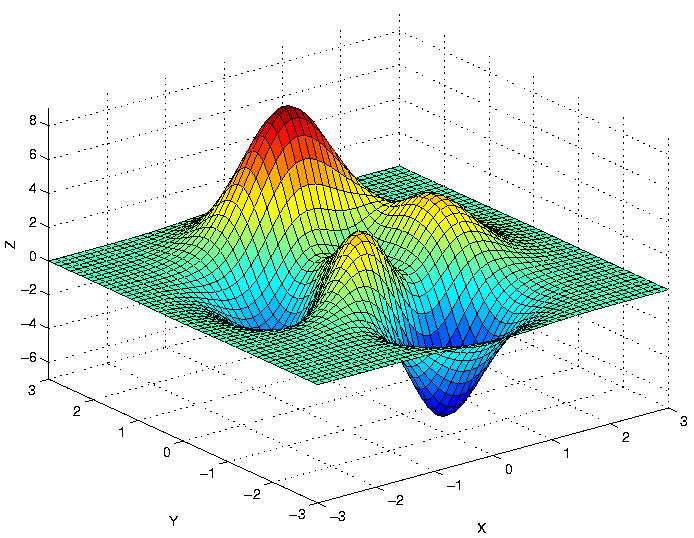
\includegraphics[width=0.45\textwidth]{Images/Gradient.png}
	\caption{\textbf{Multidimensional graph with hills and valleys} \cite{steemit}}
	\label{fig:Gradient}
\end{wrapfigure}
We can picture this visually by observing figure 2 to the right. Imagine that we have a ball at rest anywhere in this graph with a goal of reaching the lowest point in the graph. We start by finding the gradient of the spot that the ball is currently at. From this, we can determine which way is down and we also have a slope at the current point. Using both of these together we can both move down toward a lower point and at the same time we can move the ball a distance in proportion to the slope that it is currently at. As the ball gets closer to a minimum point, the slope gets smaller so the ball in turn moves slower as well. By the time the ball gets to the lowest point, it is moving very slowly. The error function previously shown allows us to determine how fast the ball should move and where it should move based on the accumulated costs of the network. The version of gradient descent used in this implementation is called Stochastic Gradient Descent and it uses small batches of around 15 inputs \--- which we refer to as mini-batches \--- in order to improve calculation time as this process would use a lot of memory to store everything if done in one large batch. Now that we've calculated our gradient and errors, the next step is to send these values back through the network to update the previous layer's nodes and their activations and weights.

\subsection{Backward Propagation}
The last element of our neural network is backward propagation which as previously stated is the act of sending errors calculated at the output layer back through the network to update weights and activations along the way. There are two main equations used to update each layer \cite{nielsen_2017}.
\begin{align}\label{eqn:backprop}
w^l &= w^l - \dfrac{\eta}{m}\delta^l(A^{l-1})\\
b^l &= b^l - \dfrac{\eta}{m}\delta^l
\end{align}
The two new variables in these equations are $\eta$ and $m$. $\eta$ is a hyperparameter for the learning rate of the network. This learning rate is a way of adjusting how big of a step the network can take. The value for $\eta$ is determined based on trial and error. $m$ is an integer representing the size of the mini-batches being trained on. These equations show how at each layer, we update the current layer's weights by taking the current layer weights then subtracting the product of passing the previous errors into the activations of the current layer. We then multiply this matrix by the scalar of the learning rate divided by the mini-batch size. This scalar helps to adjust the rate at which the weights change at each layer. Looking back at the ball rolling down a hill, this means that we slow down the rate that the ball rolls down the hill which prevents overshooting the minimum. We then perform a similar function on the bias matrix at each layer except we only subtract the scaled errors from the biases at the current layer. After both of these changes have been made, then we move on to the next layer backward until we are at the input layer again. Thus after this process completes, the network has been trained on that single set of inputs passed in. This entire process repeats for each input in the mini-bath and then a new mini-batch is passed in through this function until the entire training set of data has been used to train the network. The results of this implementation's training and testing are shown in section 4 of this paper.

\section{Implementation}
The implementation of this series of algorithms that is used in this project keeps most of the core concepts of a feed forward network as seen in section 2, however a few big features have been added in order to improve training time and accuracy of results. The first change made is that we opted to use the root mean squared algorithm RMSprop to help improve the precision of each step that the gradient descent algorithm makes while moving toward the local minimum. The next improvement that works hand in hand with RMSprop is the addition of the Nesterov Momentum algorithm which helps to improve the long term accuracy of the network by ignoring most local minima in search of the lowest point in the function\cite{ruder_2016}. We also rewrote the entire program to improve readability and restructured how each function interacts with one another in order to allow for the addition of RMSprop and Nesterov Momentum\cite{readthedocs,ruder_2016}.

\subsection{RMSprop}
RMSprop, which stands for Root Mean Squared Propagation, is a formula that normalizes the gradients calculated during gradient descent. It is a widely accepted replacement to a similar algorithm called rprop which operated using a similar structure to RMSprop however it didn't work well with a mini-batch gradient descent approach\cite{hinton}. RMSprop however, works with mini-batches and it does this by keeping track of recent gradients calculated in a rolling average\-- meaning each time a gradient is calculated, we save it into a cache array then apply a function to that array then store the new result as the most recent gradient. The following equations form the basis for RMSprop\cite{readthedocs}.
\begin{align}\label{eqn:RMSprop}
r_l &= (1-\gamma)\delta_l^2 + \gamma r_{l-1}\\
v_{l+1} &= \dfrac{\eta}{\sqrt{r_l}}\delta_l\\
\delta_{l+1} &= \delta_l - v_{l+1}
\end{align}
We see some new variables here. As usual, $l$ represents the current layer that these equations are being applied to. $\gamma$ is another hyperparameter which is usually set to one of 0.9, 0.99, or 0.999\cite{cs321n}. The value that $\gamma$ is set to is determined by trial and error. $r_l$ is a cache which is where the rolling average gradients are stored for the current layer. $v_l$ is the velocity at the current layer. These are both matrices of the same dimensions as the weight matrix at the current layer. However we do not directly implement these equations in our network since we are using a modified form of RMSprop which utilizes Nesterov Momentum which is explained in section 3.2.

\subsection{Nesterov Momentum}
Back to the example of a ball rolling down a hill. The way that this hypothetical was described previously had the ball rolling down a hill then coming to a stop as it got to the local minimum of the function. The problem that we run into with this method is that if the ball gets to a local minimum but the actual minimum of the graph is elsewhere, then the ball is stuck. 
\Needspace{0.35\textwidth}
\begin{wrapfigure}{r}{0.35\textwidth}
	\centering
	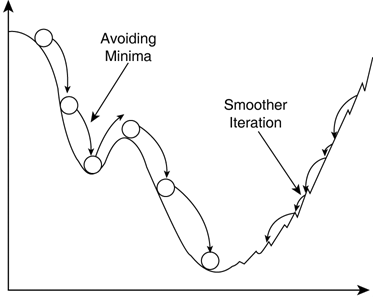
\includegraphics[width=0.35\textwidth]{Images/Momentum.png}
	\caption{\textbf{Momentum example with ball rolling out of local minima}\cite{yaldex}}
	\label{fig:Momentum}
\end{wrapfigure}
\noindent
Thus we need to implement a type of pseudo-momentum that allows the ball to continue rolling even after it has landed in a minimum point on the function. This lets the ball skip out of a shallow valley and roll into an even lower point on the graph. Notice in figure 3 that the ball rests in a local minima but since it has momentum it is able to get to the top of the next peak and continue into the next valley however since the new valley is even lower than the previous, the ball cannot roll back out of it. Another name for this formula is Nesterov Accelerated Gradient due to its nature. Since we use a mix of both Nesterov momentum and RMSprop in this implementation, we adjust the previous RMSprop equations as follows to incorporate momentum\cite{readthedocs}.
\begin{align}\label{eqn:Combined}
\delta_{l+\frac{1}{2}} &= \delta_l - \beta v_l\\
r_l &= (1-\gamma)\delta_{l+\frac{1}{2}}^2 + \gamma r_{l-1}\\
v_{l+1} &= \beta v_l + \dfrac{\eta}{\sqrt{r_l}}\delta_{l+\frac{1}{2}}\\
\delta_{l+1} &= \delta_l - v_{l+1}
\end{align}
Once again we have a new variable. $\beta$ is another hyperparameter which we've decided to set to 5.0 after testing. $\beta$ helps to scale the velocities calculated in order to force the changes made to the weights at each layer to be larger. The other new notation here is $\delta_{l+\frac{1}{2}}$. This is considered a half step in changing the weights at each layer. This is implemented using a temporary variable to store the resulting matrix so that we can use the original values later on. Other than those small changes, most of this formula is very similar to the RMSprop formula from the previous section. This equation is much easier to implement in code than it looks since most of these equations can be concatenated in order to reduce the amount of code needed. These changes can be viewed in the project code.

\section{Experiments and Results}
\subsection{System specification}
Our implementation of this neural network was designed in Windows 10 on a computer with an Intel i7 4790k CPU with 32 GB of RAM. The entire project was coded and tested in Python 3.6 using the numpy package. The graphs seen in this section are generated using the matplotlib python package.

\subsection{Dataset}
We used the MNIST data set which contains 70,000 total images of handwritten digits which were written by a wide variety of different people. This data set is split into a set of 60,000 training images which each contain the input values for each pixel in a 28 $\times$ 28 handwritten digit image and the corresponding integer value for each image. The remaining 10,000 images are used for testing purposes only and are isolated from the training images during the entire training process\cite{mnist}.

\subsection{Original Design Results}
Using the code provided in the original implementation of this algorithm\cite{nielsen_2017}, we tested many of the relationships between different input parameters such as learning rate, hidden layer count and hidden layer sizes, and mini-batch sizes. These results show a very clear relationship between these parameters as seen below. Note that each line represents a different mini-batch size as seen in the legend at the bottom right of each image. Also note that an epoch is the training of a single minibatch set. Each value is averaged over five iterations of the same parameters. 
\begin{wrapfigure}{r}{0.5\textwidth}
	\begin{minipage}{\linewidth}
	\centering\captionsetup[subfigure]{justification=centering}
	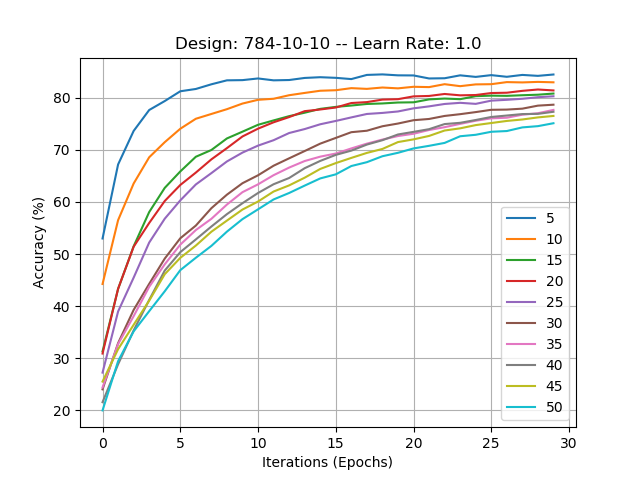
\includegraphics[width=\textwidth]{Images/Original/lr1.png}
	\subcaption{}
	\label{fig:LR1}\par\vfill
	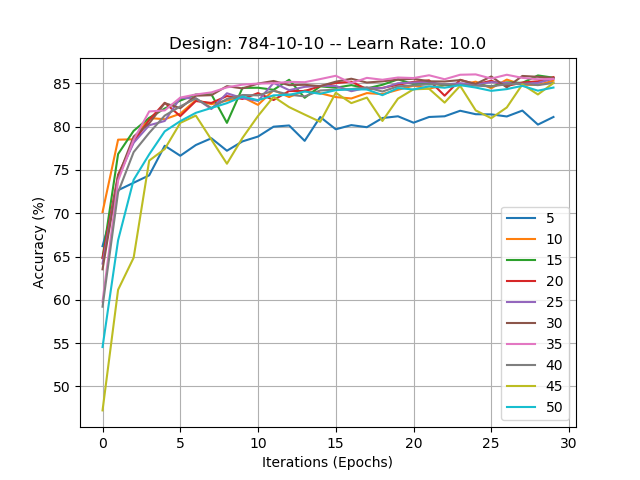
\includegraphics[width=\textwidth]{Images/Original/lr10.png}
	\subcaption{}
	\label{fig:LR10}\par\vfill
	\end{minipage}
\caption{\textbf{Original implementation results}}\label{fig:original}
\end{wrapfigure}
Both graphs in figure 4 are using the same network design of 784 nodes in the input layer, a single hidden layer of 10 nodes, and an output layer of 10 nodes. Comparing these two graphs we notice a relation between the learning rate and the stability of each training result. In figure 4(a) each line is fairly smooth and follows a predictable curve until it tapers out at 80\% \-- 82\% accuracy. If given more epochs, these values would stop increasing at 80\% \-- 83\% accuracy. Another feature to note is that each of the mini-batch lines are separated so the results are not as consistent between mini-batch sizes. We refer to this feature as the "grouping" of the lines. We can also see that mini-batch sizes between 5 and 25 items produce the best short term results. In figure 4(b) we notice a few things right away that differentiate it from figure 4(a). The most obvious difference is that the lines are much less consistent in the sense that they have many spikes and dips in accuracy over their lifetime. This is the first direct impact that an increased learning rate has on a network. Since the learning rate is much higher, then the size of steps that the network takes in the backprop process are much larger. Since these steps are much larger, then the network is constantly overshooting the minimum point then having to step backward at which point it overshoots the minimum again and this cycle repeats. Thus a larger learning rate is linked to lower precision in the gradient descent and backprop process at each step. Therefore as we lower the learning rate, the precision in each step becomes greater however this increased precision does come at cost of runtime as seen further on. The next difference in features between figure 4(a) and 4(b) is the grouping of the lines. With a higher learning rate we notice that most of the mini-batches had very close results to each other. The last feature of note is the rate at which the graphs leveled out. With the higher learning rate, the graphs got to their maximum accuracy of ~84\% within only a couple epochs whereas with a low learning rate the graphs took over 30 epochs to get beyond 80\% accuracy. Finally we notice that the most stable mini-batch sizes that produced high accuracy results were all between 10 and 30 items each. These patterns held true between many different network designs and learning rates provided. Thus we concluded that with this implementation of a neural network, as the learning rate increases so does the peak accuracy however the stability is inversely proportional to learning rate increase. We also determined that the "golden size" for mini-batches was around 10 and 25 items. Various different network designs resulted in a peak accuracy of 90\% \-- 94\%. Next we look at the runtime of a network of the same design.
\begin{wrapfigure}{r}{0.50\textwidth}
	\centering
	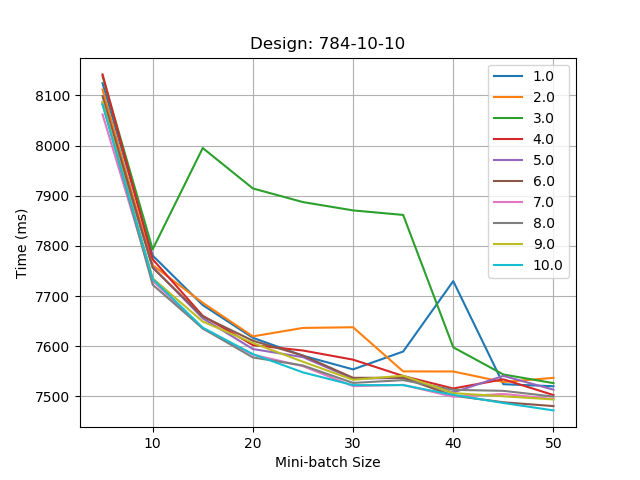
\includegraphics[width=0.50\textwidth]{Images/Original/t10.png}
	\caption{\textbf{Runtime of network with one hidden layer of 10 nodes.} Each line represents a different learning rate as seen in the legend at the top right of the graph.}
	\label{fig:T10}
\end{wrapfigure}

\noindent Figure 5 shows the graph of runtimes at different mini-batch sizes for learning rates 1 \-- 10. We can ignore the green and blue lines since they are outliers likely caused by background processes taking priority over the program as it ran. Focusing on the rest of the data, we notice that the learning rate doesn't hardly affect the runtime. The mini-batch size however affects the runtime in a very clear pattern where smaller mini-batch sizes take longer to run and larger batch sizes run much quicker. This can be attributed to the processing demand based on the mini-batch size. With smaller mini-batches, the program must run equations 5 and 6 from section 2.3 more often since there are a larger number of mini-batches to run through the backprop process. This pattern is reflected across every network design that we tested. 

\subsection{Implementation Results}
Our implementation of a feed forward neural network with RMSprop and Nesterov Momentum\cite{readthedocs,ruder_2016} shows an improvement over the original implementation both in accuracy of results and in the runtime during training. Due to the nature of a feed forward network, a single forward propagation as is performed during testing does not have any noticeable difference in runtimes. Also due to the large number of changes to both the structure and flow of the neural network in our implementation, the two networks cannot be compared with each other for most network designs. Our implementation also has a much more narrow range of network designs that will actually produce good results. Thus during testing on our implementation, our network had an input layer of 784 input nodes, three hidden layers of 30, 15, and 20 layers respectively, and an output layer of 10 nodes. Also due to the optimization algorithms added, we have a few new variables $\beta$ and $\gamma$. After many tests, we found that $\beta$ improved peak network accuracy when it was set to a value of 5.0 and $\gamma$ improved stability when set to 0.9. Also due to the way that the learning rate is implemented, a much lower value of 0.075 proved to result in a good tradeoff between stability and peak accuracy. With this network design we were able to achieve a stable accuracy of 96\% with a buffer of $\pm$1.5\% to account for fluctuation caused by the momentum algorithm. As it turned out, using a learning rate of 0.075 on the original implementation did result in its peak accuracy however it took much longer to get to that peak than with other learning rates. Thus we can compare the results of the original implementation and our implementation as seen in figure 6(a) and 6(b). 
\begin{figure}[t!]
	\centering
	\begin{subfigure}[t]{0.5\textwidth}
		\centering
		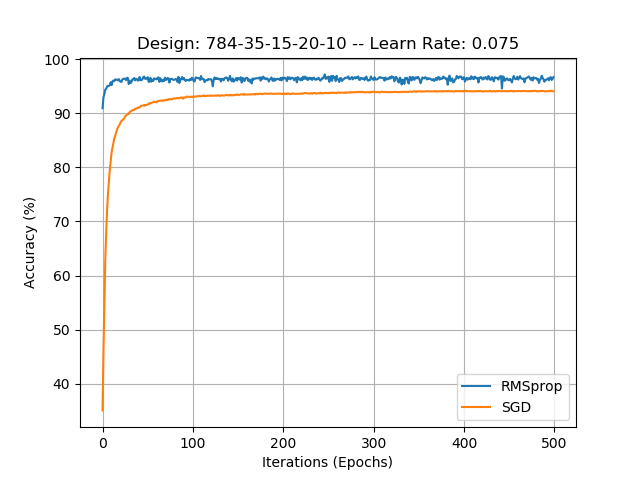
\includegraphics[width=\textwidth]{Images/New/compare1.png}
		\caption{\textbf{Comparison over 500 epochs}}
		\label{fig:Compare1}
	\end{subfigure}%
	\begin{subfigure}[t]{0.5\textwidth}
		\centering
		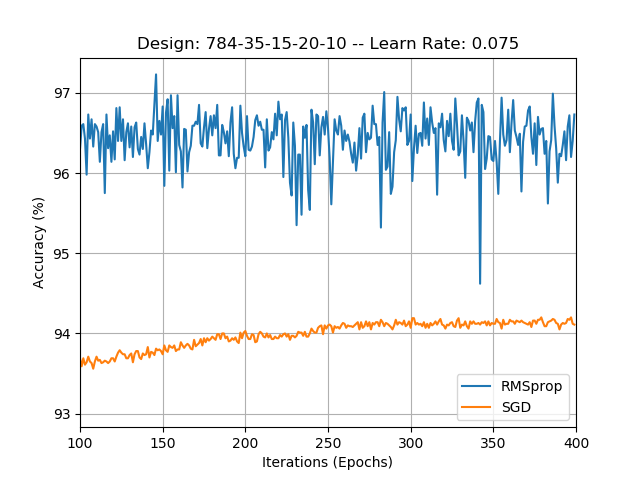
\includegraphics[width=\textwidth]{Images/New/compare2.png}
		\caption{\textbf{Zoomed in image of figure (a)}}
		\label{fig:Compare2}
	\end{subfigure}
	\caption{\textbf{Comparison of original (SGD) and our implementation (RMSprop)}}
	\label{fig:Compare}
\end{figure}

\subsection{Comparison}
From figure 6, we can see a few key patterns and differences between the original implementation using just Stochastic Gradient Descent\cite{nielsen_2017} and our implementation using RMSprop and Nesterov Momentum\cite{readthedocs,ruder_2016}. In figure 6(a), we can see that there is a big difference in the starting accuracy between both implementations. We can see that the original implementation started at around 35\% accuracy and over the course of around 200 epochs it finally leveled out at ~94\% accuracy. Our implementation started at ~92\% accuracy and quickly reached its peak at 96.5\%. In figure 6(b) we can see a close up of the difference in accuracy over time between the two implementations. We see that the original program only got a peak of ~94.15\% accuracy while our program had a peak of ~97.20\% accuracy. However as seen in 6(b) our implementation is much less stable compared to the original program. The original had a variance of about $\pm$ 0.05\% accuracy from its average while our implementation had a variance of about $\pm$ 1\% accuracy from its average with a spike of -1.5\% from its average. This difference in stability between the two algorithms is caused by the momentum in our implementation. This momentum causes the ball to continue rolling even when it has reached its final resting place. However even with this instability in our program, we were still able to get an average increase of ~2.5\% accuracy with a worst case of an increase of only ~0.5\% accuracy. We also have to count in the speed at which our implementation reaches these results. It took our program around 100 epochs less than the original in order to reach our max accuracy. In a much larger data set this could be a difference of days of training time. This brings us to the last comparison between the two implementations. In figure 6, we ran both algorithms for 500 epochs and timed the results while running as few background processes as possible to ensure results. The total runtime in seconds for each implementation is shown in table 1. We saw an improvement of over two times increased speed during training with our program. Thus not only does our implementation result in higher accuracy but it also runs over twice as fast as the original. 
\begin{table}
\caption{Runtime over 500 Epochs in Seconds}
\begin{center}
\begin{tabular}{p{0.3\textwidth}|p{0.3\textwidth}}
SGD & RMSprop w/ Momentum\\
\hline
4315.841 & 1970.499\\
\end{tabular}
\end{center}
\end{table}

\section{Applications}
Going forward, this program can be tweaked to generalize data even further in order to analyze different data sets. The way the program is set up at the moment, it can already be applied to any black and white images given the input and output layers are adjusted to accommodate for different image sizes and different classifications required. The input data could also be normalized to fit a wider range of values instead of 0 \-- 255 in order to allow for color images. Any other simple input data can be used to train this network after adjusting the layer sizes with no real trouble however in order to apply this network to different types of problems we would likely need to rewrite some of the core components. In the future we plan to rewrite this network in order to recognize sentence structure and predict conversation path based on previous conversations that the network can be trained on.

\section{Conclusion}
Pattern recognition is a difficult task for computers that is needed in order to analyze handwritten digits. Neural networks allow for computers to recognize patterns and generalize the results from training. In this paper, we analyzed an existing neural network made to classify images of handwritten digits then implemented our own design which could perform the same task. In our implementation, we used RMSprop with Nesterov Momentum\cite{readthedocs,ruder_2016} as a substitute to Stochastic Gradient Descent in order to improve both the run time and the accuracy of the neural network. Our implementation resulted in 96.5\% accuracy when classifying a set of 10,000 testing images provided by the MNIST database. These results show that neural networks can recognize patterns, a daunting task for traditional algorithms. Looking forward, this class of algorithms can be applied to much more than just handwritten digit recognition and is the future of programming.

\nocite{*}
\printbibliography


\end{document}

% Momentum
%http://www.yaldex.com/game-development/1592730043_ch18lev1sec4.html
% Gradient
%https://steemit.com/programming/@kasperfred/why-do-i-sometimes-get-better-accuracy-with-a-higher-learning-rate
% Wrapfig example
\begin{wrapfigure}{r}{0.5\textwidth}
	\centering
	\includegraphics[width=0.35\textwidth]{FFNN.jpg}
\end{wrapfigure}

% Algorithm Block Example
\begin{algorithm}
    \SetKwInOut{Input}{Input}
    \SetKwInOut{Output}{Output}

    \underline{function Euclid} $(a,b)$\;
    \Input{Two nonnegative integers $a$ and $b$}
    \Output{$\gcd(a,b)$}
    \eIf{$b=0$}
      {
        return $a$\;
      }
      {
        return Euclid$(b,a\mod b)$\;
      }
    \caption{Euclid's algorithm for finding the greatest common divisor of two nonnegative integers}
\end{algorithm}